\subsubsection{Overview}
The Actor is responsible for simulating the player's solutions to the puzzles.  The Actor will be the primary source of non-verbal information, communicating 
to the player through movement and animations. The Actor's name is Computron (for whom the game is named), and it will be seen moving around the Puzzle Scene. Computron will be tasked with manipulating the data elements of the current puzzle based on the sequence of commands that the player constructs in the Solution Pane of the User Interface.\\

Figure \ref{fig:actor_diagram} provides a high-level outline of the Actor System, all of its internal processes, and how it interacts with the other core systems of the game. \\

\begin{figure}[!htb]
  \caption{Actor Component Overview}
  \label{fig:actor_diagram}
  \centering
  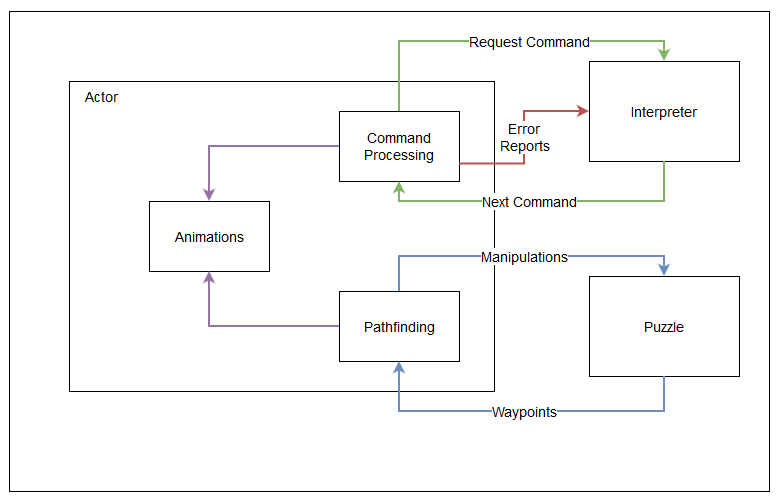
\includegraphics[scale=0.8]{Diagrams/actor_diagram.png}
\end{figure}
\newpage
The responsibilities of the Actor are as follows:

\begin{itemize}
	\item Retrieve commands from the Interpreter System
	\item Alert the Interpreter to halt execution when an invalid command is attempted
	\item Move to the correct waypoints based on the command received
	\item Properly handle data manipulation in the puzzle scene (move and update data elements
			as specified by the current command)
	\item Communicate the flow of execution to the player through visuals
	\item Illustrate to the player how data changes in response to commands
	\item Tell the player about runtime errors in their code
\end{itemize}

\subsubsection{Interpreter Interactions}
Effective integration with the Interpreter is a key component of the functionality of the Actor. The Actor relies completely on the command sequence from the Interpreter in order to illustrate the execution of the solution. If the player is using the step button to execute their solution one command at a time, the Actor waits for a signal from the Interpreter to grab the next instruction. Otherwise, the play button has been used and the Actor and Interpreter engage in that sequence of instruction retrieval and signaling automatically. The Actor will continue to retrieve the next command in sequence from the Interpreter until the sequence terminates or an invalid command is attempted. If the command can be executed, the Actor will carry out the instruction visually so that the player can understand the flow of execution and the logic behind their solution. If the command causes an error in execution, the Actor will alert the Interpreter to halt execution. The flow of this process between the Actor and Interpreter can be seen in Figure \ref{fig:interpreter_interactions}.\\

\begin{figure}[!htb]
  \caption{Interactions between the Interpreter and Actor}
  \label{fig:interpreter_interactions}
  \centering
  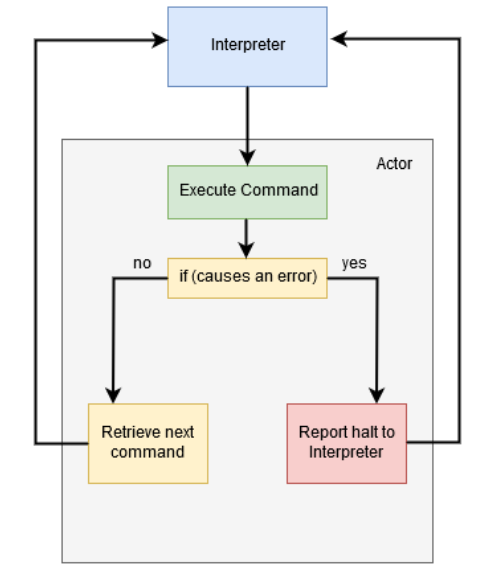
\includegraphics{Diagrams/interpreter_interactions.png}
\end{figure}

As mentioned in Section 6.7.5, there is a three step handshake between the Actor and the Interpreter when processing instructions. To summarize, the Actor requests the next command, the Interpreter responds with a data structure of that command, and the Actor then reports the results of the execution of that command to the Interpreter. Again, this communication flow can be seen in Figure \ref{fig:interpreter_Actor_interface} located in that section.\\

\subsubsection{Processing Commands}
The processing of commands is the core function of the Actor. Interfacing with the Interpreter is only the first part of command processing; the majority of that processing occurs independently within the Actor once a command has been retrieved. Figure \ref{fig:processing_commands} shows in detail how the Actor internally processes commands.\\

\begin{figure}[!htb]
  \caption{The state diagram followed by the actor when processing commands}
  \label{fig:processing_commands}
  \centering
  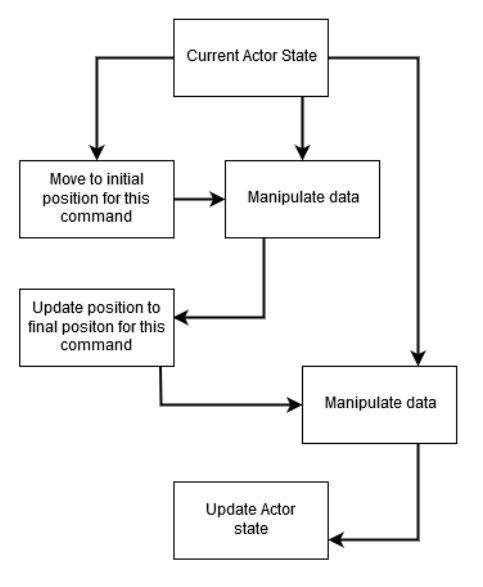
\includegraphics[scale=0.8]{Diagrams/processing_commands.png}
\end{figure}

After fetching a command, the Actor will then execute a series of movements and actions to carry out that command. This includes moving to the proper waypoint to initiate the instruction, manipulating data from the Puzzle Scene object the Actor is currently at, moving to a second waypoint to continue execution, and manipulating data at that second Puzzle Scene object. Depending on what the current command is and the status of the Actor when the new command is retrieved, some of these four steps may not be applicable. Parsing each instruction separately and successfully regardless of the current state is vital. Commands that cause errors must be reported accurately back to the Interpreter so that execution can be halted when they are encountered, and no false reporting can be tolerated. If the command won't cause an error until it is partially completed, the partial execution of that command must be shown. Additionally, commands that can complete without causing errors should always be carried out exactly as specified. This is integral to the process of the game because even if the command is the wrong selection at the time, it still needs to be executed properly in the puzzle to show the player the error in their logic. Of course, correct commands that work towards the solution also need to be executed properly to eventually reach the solved state of the puzzle.\\

The command passed from the Interpreter to the Actor needs to have several fields:
\begin{itemize}
	\item Command Opcode
	\item Command Argument
	\item Command Destination
	\item Command Description
\end{itemize}
The associated opcode for the command is an integer value unique to that command, represented by an enumerator value. Each command in the language has a corresponding opcode. By reading these values, the Actor will know which instruction type it needs to process. The argument for that command will provide additional information to the Actor, such as which Memory Card the Actor will be interacting with when it is processing a command at the Registers Waypoint. This field is nullable for commands that don't require this information. The command destination variable is a number associated with jump type commands that informs the Interpreter of where to update the Program Counter to when a jump is followed. This field is also nullable so that it doesn't effect command types that don't require it. Finally, a description of each command is included as part of the package, and is used in instruction awarding to inform the player of what each command's function is. Because this information needs to be easily passed between the Actor and Interpreter systems, it has been packaged as a class (as seen in Figure \ref{fig:command_struct}) for easier communications. \\

\begin{figure}[!htb]
  \caption{The form of the class used for packaging the fields of the Command}
  \label{fig:command_struct}
  \centering
  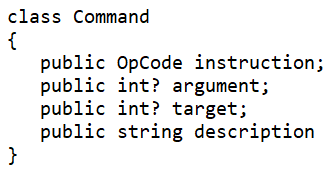
\includegraphics{command_struct.png}
\end{figure}

\subsubsection{Processing Commands}
The Actor system runs on a nested state machine. The inner level state machine is activated when a new command is received, and informs the Actor of how to behave in response to the command that is being executed. This state machine has a state for each of the 13 instructions in the CAL. Because each command has different intricacies involved in its successful execution, it was deemed necessary to allow explicit reactions to each situation. With that in mind, there are several general states that the Actor will find itself in while it is processing commands. For this reason, the command processing state machine was wrapped inside of a more general state machine that is used to dictate shared actions. The outer level state machine controls the five main action states of the Actor:
\begin{itemize}
	\item Idle
	\item Processing
	\item Moving
	\item Reporting
	\item Halted
\end{itemize}

\paragraph{Idle}~\\
The Idle state is the default position of Computron. In this state, the character sits at the resting waypoint and simply awaits for a change in state to signal it to take a different action.

\paragraph{Processing}~\\
The Processing state is used for command retrieval and parsing. This is triggered by the Interpreter when a player hits either the step or play button. The Actor then retrieves the next command from the Interpreter. If the command requires movement of the character, the Moving state is invoked. Finally, the current command state is invoked from the inner level state machine for the Actor to simulate the specific execution of that command.

\paragraph{Moving}~\\
The Moving state is only invoked if the command being processed requires movement of the character. The Actor then checks its current position against the target position for that command and if there is a large enough difference between the two positions, the position of the character is updated. The appearance of smooth movement is achieved through only checking to update the position when absolutely necessary and using the SmoothDamp feature in the Vector3 class to make motion end less abruptly.

\paragraph{Reporting}~\\
The Reporting state is invoked at the end of each command being processed. This is third part of the handshake with the Interpreter system, and involves the Actor relaying important information to the Interpreter. The first aspect is detecting an error state and accurately reporting that to the Interpreter, as well as invoking its own Halted state. If no errors were encountered, the Actor then verifies whether or not it was in stepping mode. If so, it updates its applicable control variables and awaits the next signal from the Interpreter to continue processing. If the next instruction in line is the submit instruction, though, the Actor automatically moves forward and completes the puzzle so that the player isn't required to trigger this action. If the Actor is not in the stepping mode, it passes a validation report to the Interpreter which signals the Interpreter to update the program counter appropriately and then signal the Actor to retrieve the next instruction.

\paragraph{Halted} ~\\
The Halted state is called only when an error is encountered during process. To be clear, this is the equivalent of a runtime error in the player's proposed solution, like trying to store or output a null value. Depending on what the current instruction is and the state of applicable variables, the Actor is able to report the type of error to the player via on-screen messaging.

\subsubsection{Player Messaging}
The Actor is also a key component of communication with the player. Through the visual execution of the instructions that the player has selected, the Actor conveys how the player's solution to the puzzle functions. This includes not just moving around the board and manipulating the data elements, but also providing visual cues to the user via detailed animations. For example, the data elements will be visibly picked up and held by the Actor. If that data is copied to another location, the Actor will be seen producing a copy of that data and placing it at the location specified. Data that is incremented or decremented via commands will be changed according to those commands so that the player sees and understands how the data elements are being manipulated.\\

Aside from effective visual communication, the Actor will also provide information to the player via text when applicable. For the most part, this will be explicitly in response to runtime errors that are encountered during execution. Because a certain runtime error is always the same no matter what instance of the attempted puzzle solution causes it to occur, the Actor can provide generic messaging prompts to the player about these errors independently of the puzzle itself. As previously seen in Figure \ref{fig:processing_commands}, the Actor processes the success of commands completely independently and reports those errors back to the Interpreter so that the Interpreter can halt execution. It is because of this independent evaluation that the Actor does not need to rely on input from any other systems in order to provide successful and relevant messaging on these errors.\\

In addition to error messaging, the Actor can also give puzzle specific hints to the player when requested. The hints are stored as part of each puzzle's data and are cycled through any time the player clicks on the character while it is stationary. These hints are designed to encourage the player towards a solution without giving away too much. The point is to continue to challenge the player to reach the solution on their own, but at the same time provide some guidance on where they need to concentrate their thinking.


\vfill
\clearpage